\chapter{State of the Art}

\section{Introduction}
This chapter presents the fundamental concepts necessary to understand our data center design. We first define what a data center is and its key components. Then we compare traditional Three-Tier architecture with modern Spine-Leaf architecture. Finally, we introduce the core protocols and tools used in this project.

\section{Overview of Data Centers}

\subsection{Definition and Role}
A data center is a physical facility that organizations use to house their critical applications and data. A data center's design is based on a network of computing and storage resources that enable the delivery of shared applications and data. The key components of data center design include routers, switches,\hyperref[def:firewall]{\underline{firewalls}}, servers, and application-delivery controllers~\cite{cisco}.
Its four essential components are:\\
  -\ \textbf{Compute:} Physical or virtual servers that process applications and services. In modern data centers, servers are increasingly virtualized using hypervisors such as VMware.\\
  -\ \textbf{Storage:} Systems responsible for storing data, including SAN (Storage Area Network), NAS (Network Attached Storage), and distributed storage solutions.\\
  -\ \textbf{Network:} The backbone of the data center, composed of switches, routers, and firewalls that interconnect all components and control traffic flow between them.\\
  -\ \textbf{Power and cooling:} Uninterruptible power supplies, generators, and cooling systems that ensure the physical environment remains operational at all times~\cite{dc}.\\
   
\subsection{Huawei: From Telecom Equipment Manufacturer to Data Center Leader}
Huawei is a Chinese multinational technology company founded in 1987, originally focused on telecommunications equipment before expanding into enterprise networking and cloud infrastructure. Today, Huawei is a leading provider of end-to-end data center solutions, offering switching fabrics, storage systems, and cloud platforms deployed in carrier-grade facilities worldwide~\cite{huawei}.
\section{Data Center Architectures}
\subsection{Data Center Network Architecture}
\subsection{Three-Tier Architecture}
\hyperref[def:threetier]{\underline{The three-tier}} network architecture consists of three layers: the \textbf{core layer}, which provides high-speed backbone connectivity; the \textbf{aggregation layer}, which manages traffic and network policies; and the \textbf{access layer}, where servers and storage devices connect to the network. Together, these layers improve network performance, reliability, and scalability~\cite{three}.
 \begin{figure}[htbp]
    \centering
   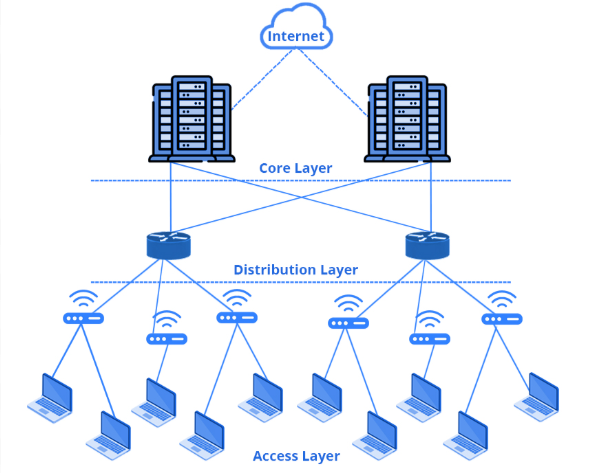
\includegraphics[width=0.5\textwidth]{figures/3tier-architecture.png}
   \caption{3-Tier Architecture}
   \label{fig:archi}
\end{figure}
\subsection{Spine-Leaf Architecture}
\hyperref[def:spineleaf]{\underline{The Spine-Leaf}} architecture is a modern two-tier model designed to overcome the limitations of the three-tier approach. It consists of spine switches that form the backbone and leaf switches that connect to end devices, with every leaf switch connected to every spine switch in a full mesh. This design guarantees that any two devices in the network are always separated by exactly two hops, delivering consistent low latency, high bandwidth, and horizontal scalability. It is widely adopted in hyperscale and cloud data centers~\cite{spine}.
\begin{figure}[htbp]
    \centering
   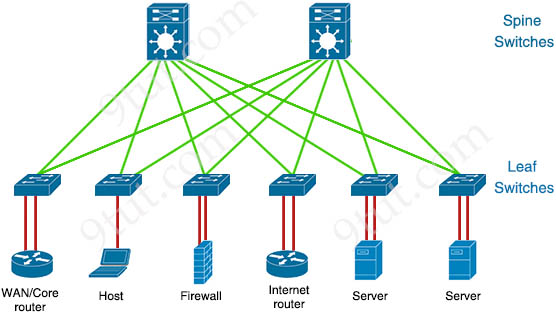
\includegraphics[width=0.5\textwidth]{figures/spine_leaf_architecture.jpg}
   \caption{Spine-Leaf Architecture}
   \label{fig:spineleaf}
\end{figure}
\section{Network Components}
\subsection{Spine Switches}
\hyperref[def:spine]{\underline{Spine switches}} form the core forwarding layer in a spine-leaf architecture. Therefore, EoR-1 and EoR-2 serve as spine switches. They connect only to leaf switches and do not connect directly to servers. Their primary role is to provide high-speed, redundant connectivity between the leaf switches, ensuring reliable and scalable traffic forwarding across the fabric.
\begin{figure}[htbp]
    \centering
   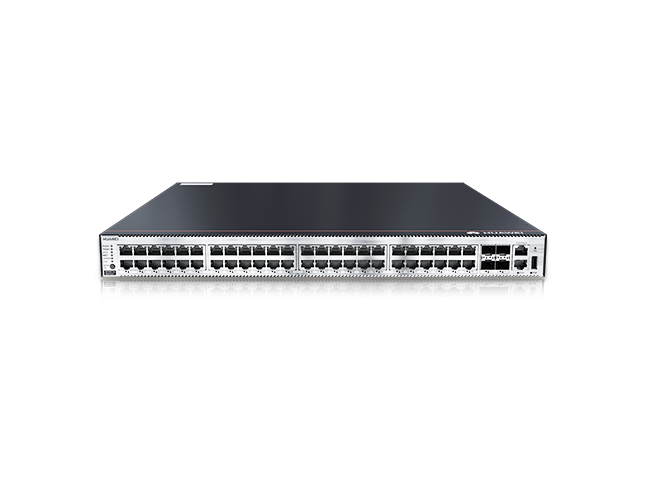
\includegraphics[width=0.3\textwidth]{figures/CloudEngine-S5731-H-v2.png}
   \caption{Huawei CloudEngine S5731 Switch Model}
   \label{fig:switch}
\end{figure}
\subsection{Leaf Switches (ToR):}
\hyperref[def:leaf]{\underline{Leaf switches}} provide server connectivity in the access layer. Positioned as Top-of-Rack switches, they connect to servers via access ports and uplink to spine switches via trunk ports. Each cabinet typically contains two leaf switches operating in active-standby mode using MLAG, with one ToR active and one standby, providing sub-second failover~\cite{switches}.
\subsection{Firewalls:}
Firewalls enforce security policies between network zones. In our design, two firewalls (FW-1 and FW-2) operate in an \hyperref[def:activestandby]{active-standby} \hyperref[def:cluster]{\underline{cluster}} at the network edge. They provide zone separation between \hyperref[def:untrust]{\underline{Untrust}} (external networks), \hyperref[def:dmz]{\underline{DMZ}}, and \hyperref[def:trust]{\underline{Trust zones}}, as well as stateful packet inspection tracking connection states. Firewalls are critical for enforcing the principle of least privilege: the DMZ can receive external traffic, but the Trust zone can only be accessed through controlled firewall rules~\cite{firewall}.
\begin{figure}[H]
    \centering
   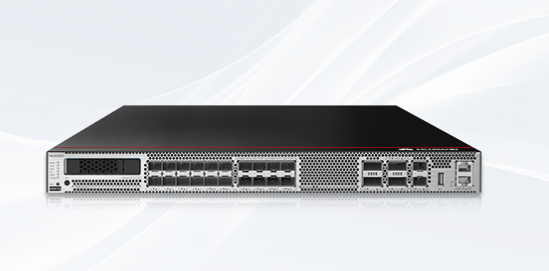
\includegraphics[width=0.3\textwidth]{figures/firewall.png}
   \caption{Huawei HiSecEngine USG6700E Firewall Model}
   \label{fig:firewall}
\end{figure}
\subsection{Servers:}
Servers host the applications and data that a data center exists to serve. The separation of management and service networks follows security best practices: administrators access management IPs for configuration, while service IPs handle application traffic. This isolation prevents management access from being exposed to the application layer~\cite{server}.
\begin{figure}[H]
    \centering
   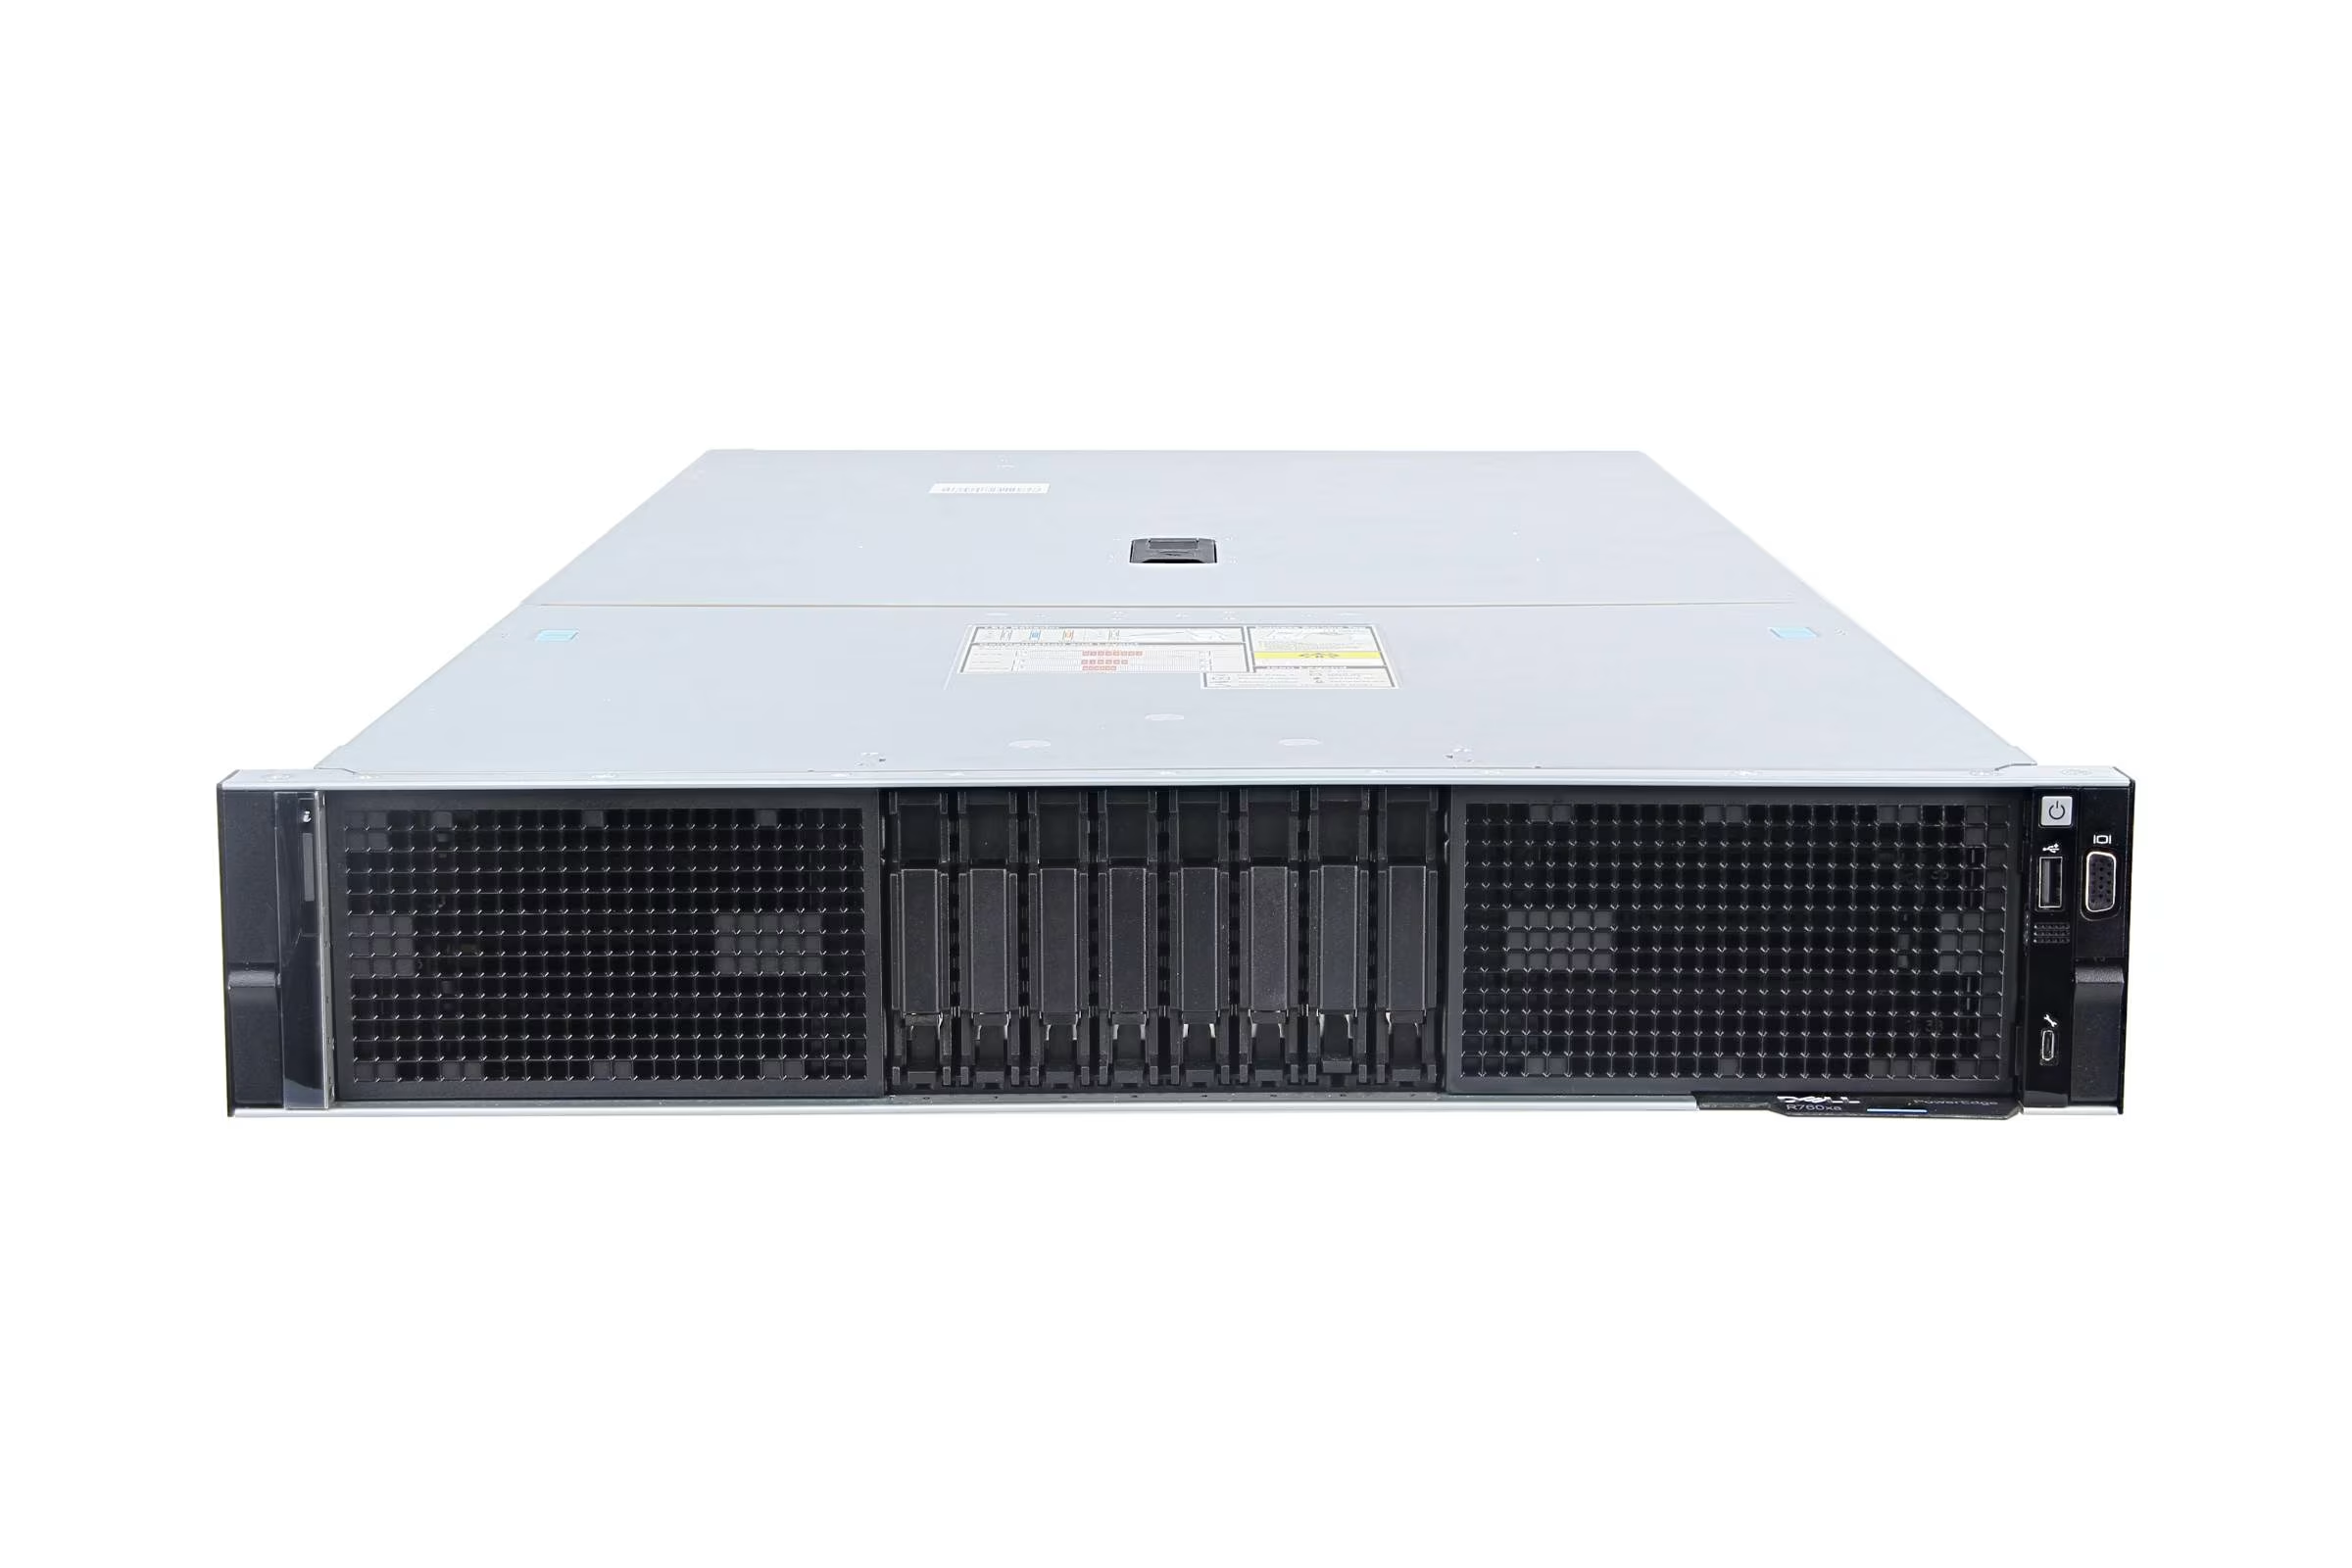
\includegraphics[width=0.3\textwidth]{figures/dell_poweredge_r760xa.png}
   \caption{Dell PowerEdge R760xa Server Model}
   \label{fig:server}
\end{figure}
\section{Core Networking Concepts}

\subsection{VLAN Segmentation and Network Zones}
A \hyperref[def:vlan]{\underline{VLAN}} logically segments a physical network into isolated broadcast domains. This improves security and reduces unnecessary traffic. In data centers, VLANs separate different traffic types such as management, storage, and application traffic. Network zones (DMZ, Trust, Untrust) extend VLAN isolation with firewall-enforced security policies. The DMZ hosts public-facing services, the Trust zone contains internal applications, and the Untrust zone represents external networks~\cite{vlan}.
\subsection{Redundancy and High Availability}
Redundancy is a fundamental principle in data center design. It ensures that the failure of a single component does not result in a service outage. In our project, redundancy is implemented at every layer of the architecture~\cite{high}:\\
  -\ \textbf{Security layer:} Two firewalls deployed in parallel, both connected to external networks and to the core switches.\\
  -\ \textbf{Spine layer:} Two EoR switches, each connected to all eight ToR switches, providing multiple forwarding paths.\\
  -\ \textbf{Leaf layer:} Each cabinet contains two ToR switches, ensuring servers remain connected even if one switch fails.\\
This multi-level redundancy guarantees high availability across the entire infrastructure using multiple protocols.
\subsection{Virtualization Principles}
Virtualization is the process of creating virtual instances of physical resources such as servers and networks. \hyperref[def:vmwareworkstation]{\underline{VMware}} is used to virtualize the IT infrastructure within each cabinet, creating virtual servers that communicate with the simulated network in \hyperref[def:pnetlab]{PNETLab}~\cite{virtu}.

\section{Conclusion}
This chapter has presented the essential concepts of modern data centers, comparing traditional Three-Tier architecture with Spine-Leaf. The analysis shows that Spine-Leaf offers consistent latency, better east-west traffic handling, and horizontal scalability, making it the preferred choice for cloud-scale infrastructures. These findings provide the theoretical basis for the design presented in the next chapter.